\documentclass[10pt,twocolumn]{article}

\usepackage[letterpaper,margin=0.72in,columnsep=0.24in]{geometry}
\usepackage{amsmath,amssymb,booktabs,graphicx,microtype}
\usepackage[dvipsnames]{xcolor}
\usepackage[round,authoryear]{natbib}
\usepackage[colorlinks=true,allcolors=MidnightBlue]{hyperref}
\usepackage{enumitem}
\usepackage{caption}
\usepackage{url}
\usepackage{dblfloatfix}
\usepackage{placeins}
\usepackage{xspace}

\setlength{\parindent}{1em}
\setlength{\parskip}{0pt}
\setlength{\textfloatsep}{8pt plus 2pt minus 2pt}
\setlength{\dbltextfloatsep}{8pt plus 2pt minus 2pt}
\setlength{\floatsep}{6pt plus 2pt minus 2pt}
\setlist{leftmargin=*,topsep=2pt,itemsep=1pt,parsep=0pt}
\captionsetup{font=small,labelfont=bf}
\setcounter{topnumber}{3}
\setcounter{bottomnumber}{2}
\setcounter{totalnumber}{5}
\setcounter{dbltopnumber}{2}
\renewcommand{\topfraction}{0.95}
\renewcommand{\bottomfraction}{0.90}
\renewcommand{\textfraction}{0.05}
\renewcommand{\floatpagefraction}{0.75}
\renewcommand{\dbltopfraction}{0.95}
\renewcommand{\dblfloatpagefraction}{0.75}

\newcommand{\ind}{\mathbb{I}}
\newcommand{\Geo}{\textsc{GeoCov}\xspace}
\newcommand{\RI}{\textsc{RI}\xspace}

\title{\textbf{GeoCov: Geometry-Aware Fixed-Budget Memory}\\
for Long-Horizon Video Generation}
\author{Anonymous authors}
\date{}

\begin{document}
\maketitle

% Working end-state abstract: VMem transfer, valid CUT3R/VBench-Long results,
% and spatial admission/duplicate-removal comparisons remain to be verified.
% The current VMem hook caps eligible views, not all persistent storage.
\begin{abstract}
Camera-controlled video generators use spatial memory to reconstruct previously
visited scenes. Existing spatial-memory systems address this by retaining the
full generated history for selective retrieval or carefully admitting new
observations to reduce redundancy. Both strategies can leave the archive
growing with generated history or explored space. This growth increases
storage requirements and, with exhaustive retrieval, lookup cost; moreover,
retaining generated observations preserves errors that can later re-enter the
conditioning context. We introduce \Geo, an online controller that maintains
a strictly bounded archive through geometry-aware eviction. \Geo constructs
a camera-pose and appearance graph and removes observations whose views are
supported by geometric and visual substitutes. With a fixed budget and chunk
size, persistent memory and per-query retrieval cost remain independent of
video duration, without retraining or modifying the generator or retriever.
Across MemCam, WorldMem, and VMem, experiments show that a small, carefully
maintained archive preserves or improves video quality, camera consistency,
and long-horizon consistency, evaluated using LPIPS, FVD, CUT3R-based camera
metrics, VBench, and VBench-Long. On fifteen matched 180-second MemCam
trajectories, \Geo retains 32 rather than 5,397 frames, reducing FVD by 35.1\%
and LPIPS from 0.5980 to 0.5876. Comparisons with spatial admission and
duplicate-removal policies demonstrate the value of reassessing which
observations remain necessary. These results challenge complete retention as
a default: effective long-horizon memory requires deciding what to forget,
not merely what to retrieve.
\end{abstract}

\section{Introduction}

A camera leaves a room, explores a hallway, and returns minutes later. A
consistent video generator should reconstruct the same room rather than invent
a new one. Because the room may no longer appear in the generator's immediate
context, camera-controlled video systems maintain spatial memories of earlier
observations and retrieve them when the camera returns
\citep{contextasmemory,memcam,worldmem,vmem}.

Two common strategies organize this history. Full-history systems retain
generated observations and select relevant evidence at retrieval time:
Context-as-Memory and MemCam use camera field-of-view (FOV) overlap to retrieve
historical frames \citep{contextasmemory,memcam}. Selectively growing spatial
archives reduce redundancy during construction. VMem merges spatial evidence
and removes older observations associated with highly similar poses
\citep{vmem}; Memory Forcing selects keyframes that reveal new regions or
provide missing historical context \citep{memoryforcing}. These construction
rules can coexist with sophisticated retrieval: AnchorWeave, for example,
selects complementary local memories to cover the next camera trajectory
\citep{anchorweave}. Selecting a compact context to read, however, does not
itself bound the archive from which that context is drawn.

Full retention makes storage grow with generated history, while selective
construction can make it grow with explored space. Suppressing repeated views
of one room does not limit the number of distinct rooms that an archive may
eventually represent. Exhaustive retrieval also becomes more expensive as
the archive expands, although spatial indices can mitigate lookup cost.
There is a separate quality concern: these observations are generated, not
ground-truth measurements. A geometrically relevant memory may contain scene
errors that are then supplied as conditioning for later generation. In our
complete-retention rollouts, selected historical indices become more
view-aligned over time while the generated content at those indices becomes
more corrupted (Fig.~\ref{fig:mechanism}). Retaining every observation is
therefore neither a storage solution nor a guarantee of useful conditioning.

We study a complementary question: \emph{which historical views should remain
available when persistent memory cannot grow?} A rule for admitting an
informative observation need not determine which existing observation to
relinquish when storage is exhausted. Moreover, an observation that originally
revealed a new region may become redundant once later views provide
substitutes. Its continued value depends on the other observations currently
available. This motivates retention based on \emph{view coverage and
substitutability}: preserve observations with little alternative support and
remove those whose views are already represented by several geometrically
nearby, visually similar memories.

We implement this principle as \emph{Geometric Coverage} (\Geo), an online
fixed-budget memory controller. At each update, \Geo combines existing and
new memories in a pose--appearance graph, scores each observation by neighbor
support and its closest substitute, and evicts low-utility items until $B$
remain. At fixed budget and chunk size, the retained archive and exact
candidate-scoring cost per query are independent of rollout length. The
controller requires no retraining or scene reconstruction and leaves the
video model, denoising schedule, and retrieval rule unchanged. It adapts the
coverage intuition behind SLAM keyframe culling \citep{orbslam,orbslam2} to
the maintenance of self-generated visual evidence. Bounded memory also
appears in long-video systems such as MemFlow and Surprise Forcing
\citep{memflow,surpriseforcing}; our focus is geometric and visual
substitutability for camera-controlled revisits, not bounded memory alone.

A strict budget necessarily trades historical availability for compactness.
We examine this tradeoff by separating \emph{retention loss}, caused by
deleting useful observations, from \emph{selection loss}, caused when the
retriever overlooks useful evidence that remains (Fig.~\ref{fig:retention-selection}).
Complete retention avoids deletion but can leave substantial evidence unused.
FIFO and rarity--irreplaceability (\RI) isolate recency and appearance-based
retention within our pipeline: FIFO loses useful history, while \RI preserves
more of it but leaves a larger selection gap than \Geo. These are controlled
policy comparisons, not reproductions of external spatial-memory systems.

\begin{figure*}[!tbp]
    \centering
    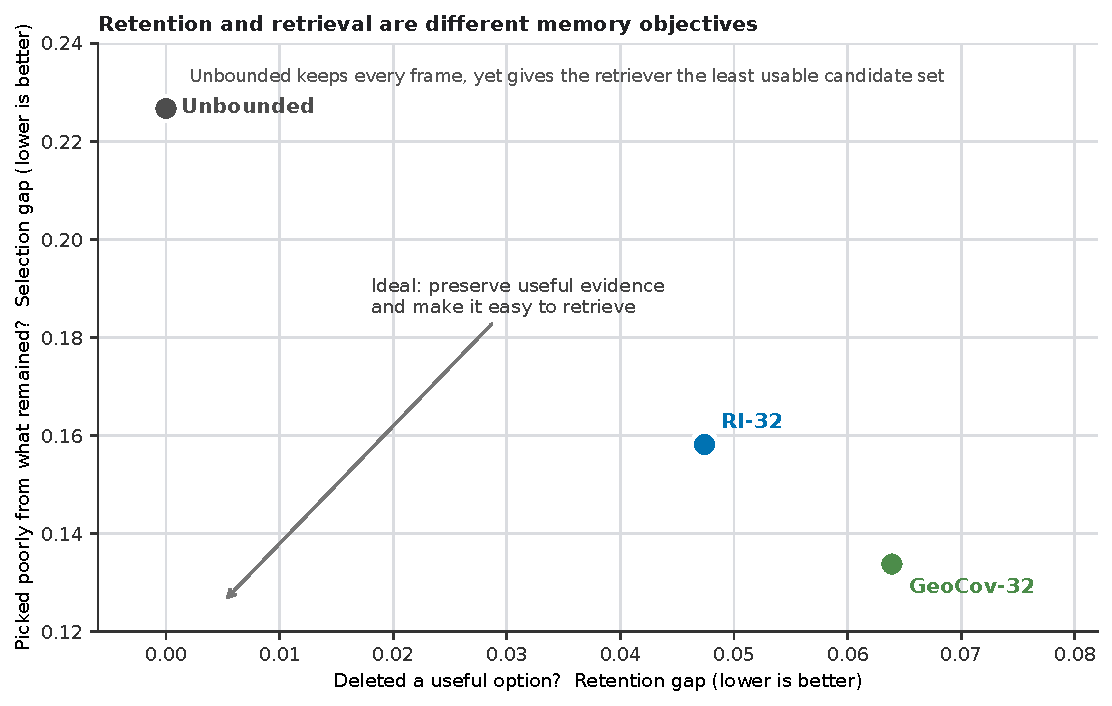
\includegraphics[width=0.94\textwidth]{figures/retention_selection_tradeoff.pdf}
    \caption{\textbf{Memory must preserve evidence and make it retrievable.}
    Retention gap measures useful history lost to deletion; selection gap
    measures the retriever's shortfall from the best retained item. Complete
    retention has no deletion loss but the largest selection gap; FIFO loses
    useful history. At matched budgets, \RI has lower retention gap than
    \Geo, while \Geo has lower selection gap. Values use common-source pixels
    on thirteen trajectories; lower-left is better.}
    \label{fig:retention-selection}
\end{figure*}

On fifteen matched 180-second MemCam trajectories, \Geo-32 retains 32 of 5,397
frames while reducing LPIPS from 0.5980 to 0.5876 and FVD from 734.2 to 476.6.
It also outperforms the tested FIFO and \RI archives on both metrics. A
corresponding controller improves LPIPS from 0.652 to 0.534 and FVD from
3077.6 to 1116.9 on fifteen 60-second WorldMem videos. These results test the
design in two generation systems. With pixels shared across policies, curated
candidate sets yield cleaner selected indices; randomly expanding a fixed
recent-history pool does not systematically lower their fidelity. The benefit
is therefore not an intrinsic penalty for candidate count. The evidence
supports deciding what remains in memory, rather than treating complete
retention as a quality upper bound.

% Add VMem transfer, measured scaling, spatial-policy comparisons, and verified
% CUT3R/VBench-Long findings here once their experiments are complete.

Our contributions are:
\begin{itemize}
    \item an online controller that uses geometric and visual substitutes to
    allocate a fixed persistent-memory budget to historical views;
    \item matched MemCam and WorldMem results showing that compact geometric
    archives can improve video quality without changing the generator or
    retriever;
    \item a retention--selection analysis, with shared-pixel and fixed-history
    controls, that examines what is lost through eviction and what remains
    usable by the retriever.
\end{itemize}

\section{Problem Setting}
\label{sec:problem}

At chunk $t$, let $P_t$ denote the known camera trajectory, $M_{t-1}$ the
persistent archive, and $N_t$ the memories produced in the new chunk. A
memory-guided generator follows
\begin{align}
    C_t &= R(P_t;M_{t-1}), \\
    \hat{Y}_t &= G(\hat{Y}_{t-1},P_t,C_t), \\
    M_t &= U(M_{t-1},N_t;B),
\end{align}
where $R$ retrieves a small context, $G$ generates the next chunk, and $U$
updates the archive. Complete retention appends $N_t$ and ignores $B$. Our
intervention changes only $U$.

Suppose each of $T$ chunks contributes $s$ candidates. Complete retention
stores $O(Ts)$ items. Exhaustive retrieval scores $O(ts)$ items at chunk $t$
and performs $O(T^2s)$ comparisons over the rollout. A fixed archive stores
$O(B)$ items and requires $O(B)$ exact comparisons per query, or $O(TB)$ over
the rollout. These are properties of the evaluated exact implementation, not
lower bounds on retrieval: approximate nearest-neighbor or pose indices can
accelerate either archive \citep{faiss}.

Complete retention is an availability oracle because it never deletes an
item. It is not a quality oracle: the retriever can overlook a useful item or
select a self-generated observation that has drifted. A bounded controller
must therefore balance two errors. Deleting too aggressively removes useful
history, while an uncurated archive can present the fixed retriever with a
poorly organized candidate set.

\section{Geometric Coverage Memory}
\label{sec:method}

\Geo operationalizes the two requirements in
Fig.~\ref{fig:retention-selection}: retain representatives of sparsely covered
views, and remove redundant alternatives where several substitutes are
available. We estimate substitutability using camera pose and visual
appearance. This gives a pose--appearance proxy for shared view coverage
without requiring a reconstructed scene.

At each update, \Geo forms the prospective archive
$V_t=M_{t-1}\cup N_t$. Item $i\in V_t$ has camera-to-world pose $(R_i,t_i)$
and a normalized DINOv2-Base descriptor $z_i$ \citep{dinov2}. Let
$\widetilde d_t$ be the median nonzero pairwise translation distance in
$V_t$, with value one if all positions coincide. We define
\begin{align}
 d_p(i,j) &=
 \frac{\lVert t_i-t_j\rVert_2}{\max(\widetilde d_t,10^{-6})}
 +2\frac{\theta(R_i^\top R_j)}{\pi}, \\
 \theta(R) &= \arccos\!\left(\operatorname{clip}
 \left(\frac{\operatorname{tr}(R)-1}{2},-1,1\right)\right), \\
 K(i,j) &= 0.65\exp[-d_p(i,j)]
 +0.35\max(z_i^\top z_j,0).
 \label{eq:affinity}
\end{align}
Pose receives most of the affinity weight; DINO separates nearby observations
whose visible content differs.

\begin{figure*}[!tbp]
    \centering
    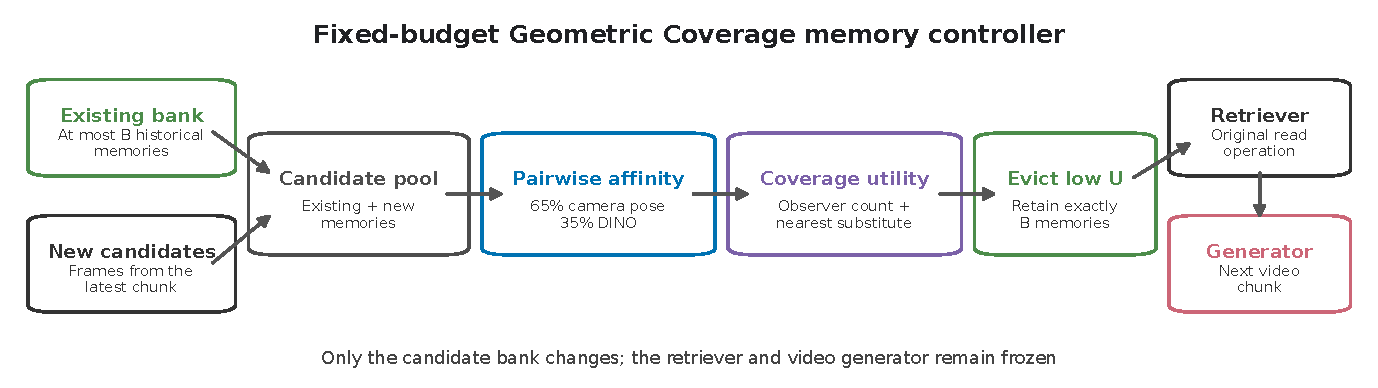
\includegraphics[width=0.96\textwidth]{figures/model_architecture.pdf}
    \caption{\textbf{Online \Geo update.} Existing and new memories form a
    pose--appearance graph. \Geo evicts locally redundant nodes to meet the
    budget; the original retriever and generator then use the curated bank.}
    \label{fig:architecture}
\end{figure*}

Let
\begin{equation}
 c_i=\sum_{j\neq i}\ind[K(i,j)\geq0.65],\qquad
 k_i^{\max}=\max_{j\neq i}K(i,j).
\end{equation}
The retention utility is
\begin{equation}
 u_i^{\mathrm{Geo}}=
 1-\min(c_i/3,1)+\frac{0.5}{c_i+1}+0.25(1-k_i^{\max}).
 \label{eq:geocov}
\end{equation}
The first two terms favor sparsely covered regions. The final term favors an
item without a close substitute. Low utility therefore identifies local
redundancy in camera and appearance space. The controller removes the
lowest-utility eligible items until $|M_t|\leq B$. Its direct implementation
builds an $O((B+s)^2)$ affinity matrix and stores $O(B)$ persistent items.

\paragraph{Protected items.}
The reported MemCam implementation reserves the initial conditioning frame in
\Geo and \RI, while complete retention contains it by construction. FIFO and
K-center do not reserve it. All bounded policies temporarily protect the newest
section endpoint during an update so that the next chunk has current local
context. Protected items count toward $B$. Section~\ref{sec:controls}
quantifies the initial-frame contribution; no future view or ground truth is
used by the controller.

\section{Experimental Setup}
\label{sec:setup}

\paragraph{MemCam.}
We use the public MemCam implementation based on the Wan2.1 1.3B diffusion
transformer \citep{wan,memcam}. The primary evaluation contains fifteen
matched 180-second trajectories from the Context-as-Memory dataset
\citep{contextasmemory}. Each rollout contains 5,397 generated frames in
76-frame target sections with 50 denoising steps. Policies share checkpoints,
prompts, camera paths, and seeds. The primary budget is $B=32$; we also test
$B\in\{16,64,128\}$.

\paragraph{WorldMem.}
We evaluate the first fifteen matched 60-second WorldMem videos using its
latent-memory interface \citep{worldmem}. The geometric controller is adapted
to the stored representation while keeping the same view-coverage principle.
Results are compared only within WorldMem.

\paragraph{Baselines.}
Complete retention keeps the full history. FIFO retains the most recent $B$
items. K-center maintains descriptor coverage. Marginal Coverage Eviction
(MCE) approximates a facility-style objective. Rarity--irreplaceability (\RI)
clusters DINO features and favors small appearance clusters whose members lack
an RGB substitute. These policies test full availability, recency, generic
diversity, marginal coverage, and appearance rarity. All use the original
system retriever after archive construction.

\paragraph{Metrics.}
LPIPS \citep{lpips} compares generated frames with trajectory-indexed ground
truth. FVD \citep{fvd} uses the same StyleGAN-V I3D detector, 16-frame clips,
four clips per video, stride four, and 224-pixel inputs within each comparison.
Standard VBench \citep{vbench} measures subject and background consistency,
motion smoothness, dynamic degree, aesthetics, and imaging quality. PSNR,
SSIM \citep{ssim}, and DINO distance \citep{dinov2} are used only for memory
diagnostics. Diagnostic confidence intervals bootstrap trajectory-level means.

\paragraph{Evaluation scope.}
The policy family and constants were developed while inspecting the MemCam
suite, so those trajectories are not an untouched test set. WorldMem changes
the backbone and memory interface but was evaluated after MemCam. Headline
LPIPS, FVD, and VBench values are matched point estimates over fifteen videos;
we do not claim statistical significance for them. CUT3R \citep{cut3r} is
excluded after its evaluator failed a ground-truth camera sanity check;
VBench-Long is excluded because its evaluation is incomplete.

\section{Results}
\label{sec:results}

\subsection{Long-horizon video quality}

\begin{table}[!htbp]
\centering
\caption{Matched 180-second MemCam results. All bounded policies use $B=32$;
lower is better.}
\label{tab:main-quality}
\small
\begin{tabular}{lrrr}
\toprule
Policy & Stored & LPIPS $\downarrow$ & FVD $\downarrow$ \\
\midrule
Complete retention & 5,397 & 0.5980 & 734.2 \\
FIFO & 32 & 0.6514 & 677.3 \\
\RI & 32 & 0.5939 & 550.4 \\
\Geo & 32 & \textbf{0.5876} & \textbf{476.6} \\
\bottomrule
\end{tabular}
\end{table}

Table~\ref{tab:main-quality} presents the primary result. Relative to complete
retention, \Geo reduces FVD by 35.1\% and LPIPS by 0.0104 while retaining
0.59\% of the frames. \RI also improves both metrics but remains behind
\Geo. FIFO improves FVD and substantially worsens LPIPS, showing that the
tested gain does not follow from using a small recent-history bank.

\begin{figure}[!tbp]
    \centering
    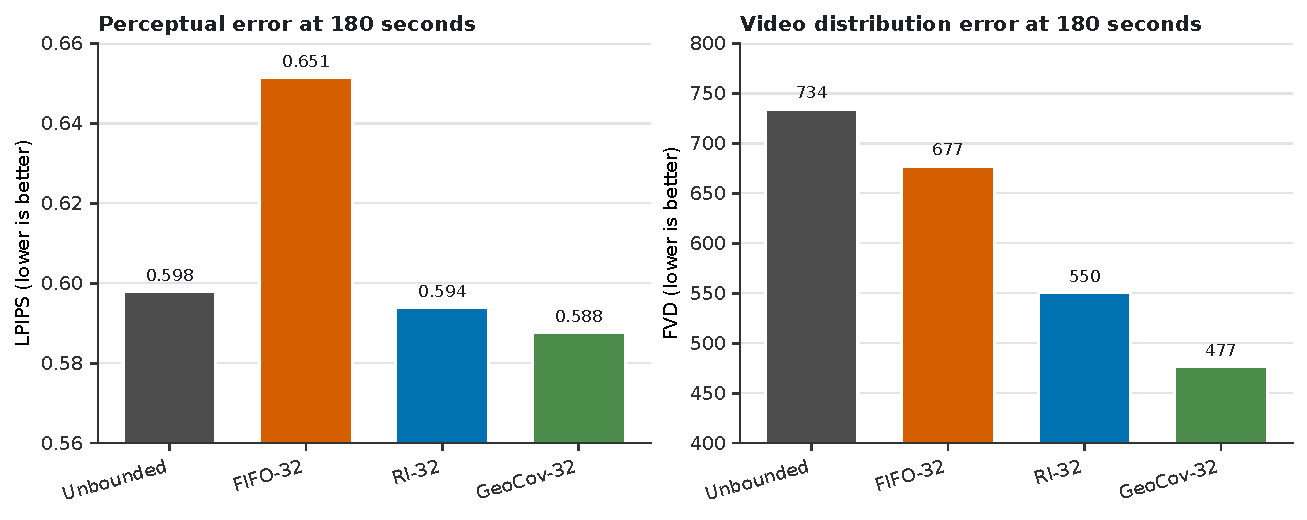
\includegraphics[width=\columnwidth]{figures/quality_180s.pdf}
    \caption{\textbf{MemCam quality at 180 seconds.} Structured B32 archives
    improve LPIPS and FVD over complete retention; FIFO does not reproduce the
    same result.}
    \label{fig:quality}
\end{figure}

\begin{table}[!htbp]
\centering
\caption{Matched 60-second WorldMem results at $B=32$. Values are comparable
only within WorldMem; lower is better.}
\label{tab:worldmem}
\small
\begin{tabular}{lrr}
\toprule
Policy & LPIPS $\downarrow$ & FVD $\downarrow$ \\
\midrule
Complete retention & 0.652 & 3077.6 \\
FIFO & 0.689 & 3554.9 \\
Latent-\RI & 0.546 & 1160.4 \\
Geometric Coverage & \textbf{0.534} & \textbf{1116.9} \\
\bottomrule
\end{tabular}
\end{table}

The same ordering appears in WorldMem (Table~\ref{tab:worldmem}). Geometric
Coverage improves LPIPS by 0.118 and FVD by 1960.7 relative to complete
retention. This result supports the bounded geometric principle under a second
backbone and memory interface; it does not imply that the exact MemCam score is
universally optimal.

\subsection{Budget sensitivity}

\begin{table}[!htbp]
\centering
\caption{\Geo across tested budgets. MemCam values use 180-second rollouts;
WorldMem values use 60-second videos. Lower is better.}
\label{tab:geo-budget}
\small
\begin{tabular}{rrrr}
\toprule
& \multicolumn{2}{c}{MemCam} & WorldMem \\
\cmidrule(lr){2-3}\cmidrule(lr){4-4}
$B$ & LPIPS & FVD & LPIPS \\
\midrule
16  & 0.5876 & \textbf{446.1} & \textbf{0.525} \\
32  & 0.5876 & 476.6 & 0.534 \\
64  & \textbf{0.5865} & 493.9 & 0.545 \\
128 & 0.5913 & 515.5 & 0.577 \\
\bottomrule
\end{tabular}
\end{table}

The result is not isolated to B32 (Table~\ref{tab:geo-budget}). MemCam LPIPS
is stable from B16 through B64, and every tested \Geo budget improves FVD over
complete retention. WorldMem LPIPS also remains better than complete retention
through B128. Larger is not consistently better within this policy family, so
we treat $B$ as a system parameter rather than claim a universal optimum.

\subsection{Testing coverage and retrieval}
\label{sec:gaps}

For target $q$, let $d(i,q)$ be the DINO distance between generated memory $i$
and exact-index target ground truth. Let $\mathcal{H}$ be complete history,
$M$ a policy archive, $i_M^*=\arg\min_{i\in M}d(i,q)$ the hindsight-best
retained item, and $i_R$ the item chosen by the real retriever. We define
\begin{align}
 \Delta_{\mathrm{ret}} &= d(i_M^*,q)-\min_{i\in\mathcal{H}}d(i,q), \\
 \Delta_{\mathrm{sel}} &= d(i_R,q)-d(i_M^*,q).
 \label{eq:gaps}
\end{align}
Retention gap measures quality lost by deletion. Selection gap measures
quality present in the archive but unused by the retriever. Both require
ground truth and are diagnostics, not runtime objectives.

\begin{table}[!htbp]
\centering
\caption{Common-source gaps at B32 on thirteen trajectories. Lower is better.}
\label{tab:gaps}
\small
\begin{tabular}{lrr}
\toprule
Policy & Retention gap & Selection gap \\
\midrule
Complete retention & 0.0000 & 0.2188 \\
FIFO & 0.1668 & \textbf{0.0646} \\
\RI & \textbf{0.0399} & 0.1609 \\
\Geo & 0.0426 & 0.1470 \\
\bottomrule
\end{tabular}
\end{table}

Complete retention has zero retention gap by definition but the largest
selection gap (Table~\ref{tab:gaps}). FIFO creates an easy selection problem by
discarding distant history, at the cost of the largest retention gap. \RI and
\Geo preserve substantially more useful history while reducing the selection
gap relative to complete retention. At B32, \Geo gives up 0.0027 retention gap
relative to \RI and gains 0.0139 selection gap.

Every measured increase from B16 to B128 lowers retention gap and raises
selection gap (Fig.~\ref{fig:retention-selection}). For \Geo, their sum is
0.1706, 0.1896, 0.1962, and 0.2081 at B16, B32, B64, and B128, respectively,
versus 0.2188 for complete retention. The archive can contain better evidence
without making that evidence easier for a fixed retriever to use.

\subsection{Common-source selection control}
\label{sec:common-source}

Independent policy rollouts contain different pixels because an early memory
choice changes later generation. To isolate archive composition, we reconstruct
each policy's candidate set and selected indices but load every candidate image
from the same complete-retention rollout. Each selected image is compared with
ground truth at its own historical index. Thus the pixels are fixed; only the
candidate sets and selected identities differ.

\begin{table}[!htbp]
\centering
\caption{Common-source selected-frame fidelity on fifteen trajectories.
Deltas are relative to complete retention; positive is better.}
\label{tab:common-source}
\small
\begin{tabular}{lrrr}
\toprule
Selector & PSNR & $\Delta$PSNR & $\Delta$SSIM \\
\midrule
Complete retention & 11.703 & -- & -- \\
FIFO & 11.487 & -0.216 & -0.0109 \\
\RI & 13.478 & +1.775 & +0.0672 \\
\Geo & \textbf{16.332} & \textbf{+4.629} & \textbf{+0.1512} \\
\bottomrule
\end{tabular}
\end{table}

\Geo improves PSNR by 4.629 dB (95\% CI $[3.521,5.874]$) and SSIM by 0.1512
(CI $[0.1100,0.1929]$), with positive differences on all fifteen trajectories.
\RI improves PSNR by 1.775 dB (CI $[1.005,2.683]$) and SSIM by 0.0672 (CI
$[0.0456,0.0926]$). FIFO is worse. Because the source pixels are shared,
these differences arise from which historical indices the unchanged retriever
selects from each candidate set.

\begin{figure*}[!tbp]
    \centering
    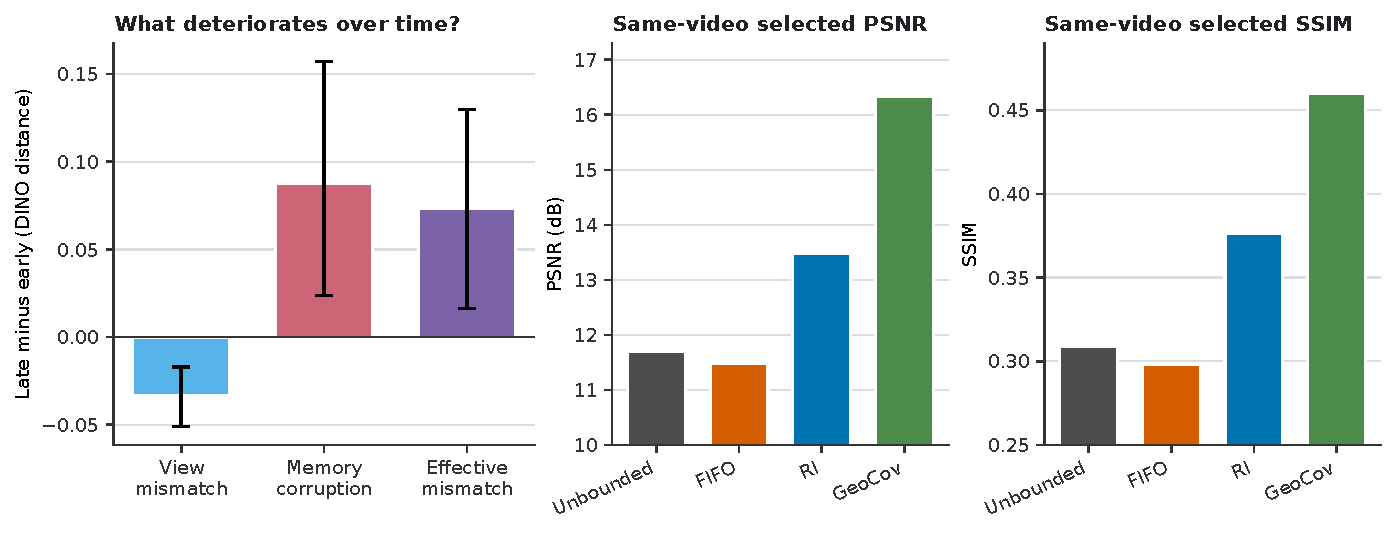
\includegraphics[width=0.78\textwidth]{figures/mechanism_evidence.pdf}
    \caption{\textbf{Selected-memory evidence.} Complete-retention selections
    move away from the hindsight-best available item as their generated
    content degrades (a--b). With candidate pixels fixed, structured archives
    lead the retriever to cleaner historical indices (c--d). Error bars are
    trajectory-bootstrap 95\% intervals.}
    \label{fig:mechanism}
\end{figure*}

The temporal analysis in Fig.~\ref{fig:mechanism} helps explain what the
retriever encounters. Across 4,200 queries, selected historical indices become
more view-aligned from early to late rollout: DINO view mismatch changes by
$-0.0335$ (CI $[-0.0511,-0.0171]$). Yet corruption of the generated content at
those indices increases by 0.0873 (CI $[0.0236,0.1572]$), and effective
mismatch to the target increases by 0.0732 (CI $[0.0165,0.1296]$). The
hindsight-best archive mismatch remains approximately flat. This analysis is
descriptive because archive composition, observation age, and rollout time
co-vary.

\subsection{Controls on initial-frame use and archive size}
\label{sec:controls}

The initial conditioning frame is the only ground-truth image stored in the
MemCam archive. Both \Geo and complete retention contain it, but curation can
change whether the retriever ranks it first. Among 9,927 queries where their
selections disagree, \Geo chooses the initial frame 1,483 times (14.9\%).
Removing those cases leaves a gain of 1.060 dB PSNR (CI $[0.213,2.290]$) and
0.0449 SSIM (CI $[0.0079,0.0900]$). On the stricter subset where neither
selection is the initial frame and both have logged FOV overlap of at least
0.80, the difference is 0.103 dB (CI $[-0.202,0.407]$) and 0.0098 SSIM (CI
$[-0.0029,0.0258]$). Thus initial-frame retrieval explains part, but not all,
of the aggregate common-source result; the high-overlap non-initial subset is
not statistically distinguishable from zero.

\begin{table}[!htbp]
\centering
\caption{Fixed-history candidate-count intervention. Winner change is relative
to the shared B32 core.}
\label{tab:fixed-pool}
\small
\begin{tabular}{lrrr}
\toprule
Pool & PSNR $\uparrow$ & SSIM $\uparrow$ & Winner change \\
\midrule
B32 & 11.275 & 0.3064 & 0.000 \\
B64 & 11.348 & 0.3025 & 0.397 \\
B128 & 11.322 & 0.3013 & 0.497 \\
B256 & 11.310 & 0.3012 & 0.581 \\
B512 & 11.330 & 0.3023 & 0.611 \\
B1024 & 11.436 & 0.3068 & 0.661 \\
All (3,797 mean) & 11.502 & 0.3075 & 0.722 \\
\bottomrule
\end{tabular}
\end{table}

The common-source policies differ in both composition and size, so we isolate
cardinality with fixed generated history and nested candidate pools. Each query
starts from the same recent B32 core; older frames are added in four random
orders while candidate pixels, camera poses, targets, and FOV scores remain
fixed. Full history changes the B32 winner in 72.2\% of queries but changes
PSNR by $+0.228$ dB (CI $[-0.109,0.664]$) and SSIM by $+0.0011$ (CI
$[-0.0117,0.0188]$). Candidate count strongly affects identity, but this
intervention provides no evidence that count alone lowers fidelity. Combined
with Table~\ref{tab:common-source}, it points to structured composition.

\section{Related Work}

\paragraph{Long-horizon video memory.}
Context-as-Memory stores historical RGB frames and retrieves them by camera FOV
overlap \citep{contextasmemory}. MemCam adds context compression and provides
an open implementation of RGB-frame retrieval \citep{memcam}. WorldMem stores
visual memories with pose and time state and reads them through learned memory
attention \citep{worldmem}. VMem indexes prior views with surfels
\citep{vmem}; Spatia maintains an updatable point cloud \citep{spatia}; Mirage
stores spatial evidence in diffusion latent space \citep{mirage}; and
AnchorWeave retrieves local geometric memories \citep{anchorweave}. We study
the persistent candidate archive that precedes these bounded reads.

\paragraph{Selective context and keyframes.}
FramePack allocates a fixed context length using frame-importance-based
compression \citep{framepack}. MemFlow combines semantic retrieval with a
prototype from the preceding chunk and sparse token activation
\citep{memflow}. We target persistent archive composition under a camera-driven
retriever; our FIFO and \RI comparisons isolate recency and appearance criteria
within that setting rather than reproduce these full systems.
SLAM systems use co-visibility graphs and keyframe culling to remove redundant
observations while preserving a map \citep{orbslam,orbslam2}. \Geo adapts this
principle to recurrent video generation, where observations are self-generated
and memory conditions a diffusion model rather than a geometric optimizer.
Surprise Forcing uses novelty, feedback-controlled
admission, replacement, and routing \citep{surpriseforcing}. Streaming subset
selection supplies broader coverage objectives \citep{nemhauser1978,
badanidiyuru2014}. Our baselines include recency, K-center, appearance rarity,
and marginal coverage.

\section{Discussion and Limitations}
\label{sec:limitations}

The design implication is that archive construction should account for both
what evidence survives and what the retriever selects. Complete retention
maximizes availability; the tested recency and rarity criteria make different
tradeoffs between retention and selection. \Geo uses view coverage and
substitutability to balance these requirements, improving the reported quality
metrics in two systems while bounding the archive. The shared-pixel and
fixed-history controls support the role of composition in those selections.

The evidence does not show that \Geo detects corrupted images. Its score uses
pose and appearance redundancy, not a calibrated quality estimate. The
common-source analysis also does not prove that selected-frame fidelity causes
the full FVD difference; a multi-trajectory content-replacement replay would
test that link more directly. Because initial-frame reservation differs across
some bounded baselines, symmetric pin/no-pin closed-loop runs remain an
important control.

Finally, the MemCam constants were developed on the reported suite, the sample
contains fifteen trajectories, and headline metrics lack matched uncertainty.
WorldMem provides a second backbone but not an untouched development process.
We have not measured matched end-to-end latency or peak memory, and the
long-duration resource values in Appendix~\ref{app:scaling} are extrapolations.
A neutral reservoir baseline, frozen evaluation on new trajectories, and FVD
estimates over a larger sample would strengthen the empirical claim.

\section{Conclusion}

An effective video memory must preserve useful views and make them available
to the retriever. Our analysis identifies retention and selection failures in
complete-history, recency, and appearance-based archives. \Geo addresses these
requirements through geometric and visual substitutability: sparsely covered
views remain valuable, while redundant observations are removed to meet a
fixed budget. It improves the reported MemCam and WorldMem quality metrics
through the original generation and retrieval interfaces. The results support
view coverage as a practical principle for constructing long-horizon video
memory.

% Start supplementary material with a fresh float queue and full-width tables.
\onecolumn
\appendix
\raggedbottom
\setlength{\intextsep}{8pt plus 2pt minus 2pt}

\section{Video-Quality Ablations}

\begin{table}[!htbp]
\centering
\caption{Matched 60-second MemCam ablation at $B=32$. Lower is better for LPIPS
and FVD; higher is better for the VBench dimensions.}
\label{tab:rarity}
\small
\resizebox{\textwidth}{!}{%
\begin{tabular}{lrrrrrrrrrr}
\toprule
Policy & LPIPS-10 & FVD-10 & LPIPS-60 & FVD-60 & Subject & Background & Motion & Dynamic & Aesthetic & Imaging \\
\midrule
\Geo & 0.4964 & 719.3 & 0.5850 & 690.5 & \textbf{0.8187} & \textbf{0.9071} & 0.9914 & 1.000 & \textbf{0.4792} & \textbf{0.5294} \\
Rarity only & \textbf{0.4878} & \textbf{682.2} & 0.5986 & 732.3 & 0.8008 & 0.8996 & \textbf{0.9925} & 1.000 & 0.4495 & 0.4976 \\
0.75 Geo + 0.25 rarity & 0.4927 & 713.1 & 0.5872 & \textbf{676.4} & 0.8104 & 0.9006 & 0.9922 & 1.000 & 0.4554 & 0.5027 \\
0.75 Geo + 0.25 RI & 0.4906 & 711.1 & \textbf{0.5825} & 691.7 & 0.8111 & 0.9000 & 0.9921 & 1.000 & 0.4589 & 0.5020 \\
\bottomrule
\end{tabular}}
\end{table}

Rarity-only performs best at 10 seconds but degrades at 60 seconds. Adding
25\% rarity gives the best 60-second FVD, while adding \RI gives the best
60-second LPIPS. Both blends reduce subject consistency, background
consistency, aesthetics, and imaging quality relative to \Geo. No composite
dominates the complete metric suite, so the final method retains the simpler
geometric score.

\section{Selected-Memory Quality}

\begin{table}[!htbp]
\centering
\caption{Selected-memory quality on each policy's own 180-second rollout.
Higher is better; ``Late'' is the final temporal portion.}
\small
\begin{tabular}{lrrrrrr}
\toprule
Policy & Selected PSNR & Selected SSIM & Late PSNR & Late SSIM & Next PSNR & Next SSIM \\
\midrule
Complete retention & 11.703 & 0.3089 & 11.433 & 0.3146 & 11.308 & 0.3082 \\
FIFO-32 & 10.619 & 0.2617 & 10.135 & 0.2546 & 10.113 & 0.2543 \\
\RI-32 & 13.396 & 0.3830 & 12.896 & 0.3723 & 11.323 & 0.3203 \\
\Geo-32 & 16.522 & 0.4759 & 15.119 & 0.4386 & 11.569 & 0.3253 \\
\bottomrule
\end{tabular}
\end{table}

Relative to complete retention, selected-frame differences are +1.693 dB PSNR
and +0.0741 SSIM for \RI, and +4.819 dB and +0.1670 for \Geo. Late next-chunk
SSIM improves by 0.0133 for \RI (CI $[0.0028,0.0279]$) and 0.0169 for \Geo
(CI $[0.0012,0.0392]$); next-chunk PSNR intervals cross zero. This analysis is
observational because earlier policy decisions change later pixels.

\section{Full Retention--Selection Sweep}

\begin{table}[!htbp]
\centering
\caption{Common-source budget sweep on thirteen matched trajectories. Lower is
better.}
\small
\begin{tabular}{lrrrrrrrr}
\toprule
& \multicolumn{2}{c}{B16} & \multicolumn{2}{c}{B32} &
\multicolumn{2}{c}{B64} & \multicolumn{2}{c}{B128} \\
Policy & Ret. & Sel. & Ret. & Sel. & Ret. & Sel. & Ret. & Sel. \\
\midrule
FIFO & .1872 & .0448 & .1668 & .0646 & .1429 & .0867 & .1203 & .1084 \\
\RI & .0583 & .1339 & .0399 & .1609 & .0317 & .1748 & -- & -- \\
\Geo & .0669 & .1037 & .0426 & .1470 & .0366 & .1596 & .0298 & .1783 \\
\bottomrule
\end{tabular}
\end{table}

Complete retention has retention gap 0 and selection gap 0.2188. Every measured
budget increase lowers retention gap and raises selection gap. \RI-B128 is
omitted because the common matched set lacks the required traces.

\section{Implementation Scaling}
\label{app:scaling}

The decoded RGB archive occupies approximately 0.38 GB at 10 seconds and 2.30
GB at 60 seconds in the evaluated MemCam implementation. Extrapolations reach
22.7 GB at 10 minutes and 136 GB at 60 minutes. Corresponding cumulative
exhaustive-retrieval estimates are 12 minutes, 20.9 hours, and 31.5 days. The
long-duration values depend on the implementation and hardware and are not
direct measurements. They illustrate bounded-state scaling, not a claim that
exhaustive search is the only possible design.

\clearpage
\section{WorldMem Budget Sensitivity}

\begin{table}[!htbp]
\centering
\caption{WorldMem 60-second LPIPS on the first fifteen matched videos. Complete
retention obtains 0.652; lower is better.}
\small
\begin{tabular}{lrrrr}
\toprule
Policy & B16 & B32 & B64 & B128 \\
\midrule
FIFO & 0.717 & 0.689 & 0.688 & 0.647 \\
Latent-\RI & 0.566 & 0.546 & 0.549 & 0.567 \\
Geometric Coverage & \textbf{0.525} & \textbf{0.534} & \textbf{0.545} & 0.577 \\
K-center & 0.545 & 0.559 & 0.575 & \textbf{0.559} \\
MCE & 0.576 & 0.575 & 0.596 & 0.604 \\
\bottomrule
\end{tabular}
\end{table}

Selected matched FVD values at B32 are 1116.9 for Geometric Coverage, 1160.4
for Latent-\RI, 3077.6 for complete retention, and 3554.9 for FIFO. Absolute
WorldMem FVD is not compared with MemCam because the systems and evaluation
sources differ.

\section{Reliability Probes}
\label{app:reliability}

\begin{table}[!hbp]
\centering
\caption{Held-out online reliability signals. AUC predicts bottom-20\%
exact-index PSNR--SSIM fidelity.}
\small
\begin{tabular}{lrrrr}
\toprule
Signal & AUC & Precision & Recall & Clean reject \\
\midrule
Unclipped fraction & 0.630 & -- & 0.183 & 0.125 \\
MUSIQ/PAQ2PIQ & 0.516 & -- & 0.314 & 0.307 \\
Raw context similarity & 0.546 & 0.294 & 0.245 & 0.151 \\
Pose-conditioned residual & 0.511 & 0.207 & 0.119 & 0.117 \\
Anchor-chain score & 0.463 & -- & 0.000 & 0.000 \\
\bottomrule
\end{tabular}
\end{table}

Generic image-quality signals use only the generated frame; context and chain
signals also use causal trace identity and camera geometry. Ground truth is
used only for held-out labels and calibration. None of these signals is
reliable enough to add to Eq.~\ref{eq:geocov}. A related offline observation
also fails to produce a useful controller: older same-view memories are cleaner
than later rewrites by 0.860 dB PSNR and 0.0397 SSIM over 823 pairs, but hard
hysteresis worsens 60-second FVD from 690.5 to 768.7 and loses four VBench
dimensions.

\section{Other Negative Results}

Density-balanced coverage obtains LPIPS/FVD 0.5941/750.3 at 60 seconds versus
0.5850/690.5 for \Geo. A 50/50 \Geo--\RI blend does not beat both
constituents. MCE, trajectory coverage, and facility-style objectives also
fail to improve the complete metric suite.

Several diagnostic hypotheses are unsupported. MemCam retrieves a fixed-size
context before denoising, so the archive does not directly enlarge the
denoiser's attention input. FOV-overlap hit rate is 100\% at thresholds 0.01
and 0.1, with median selected overlap 0.9335, making frequent zero-overlap
fallback an unlikely explanation. The largest repeated-frame share averages
0.172 and decreases with
pool size ($\rho=-0.314$). Increasing Monte Carlo FOV sampling changes 39.1\%
of winners but yields mean appearance cost 0.0029, with fewer flips in larger
pools. Finally, average archive corruption is not monotonic; deterioration is
concentrated in the query-conditioned selected subset.

\section{Preliminary Context Replay}

One valid replay holds the model, prompt, trajectory, seed, complete archive,
and preceding contexts fixed, then substitutes \Geo-selected context identities
at one late section. LPIPS changes by $-0.00177$ and DINO distance by
$-0.01691$. The direction is consistent with better conditioning, but $n=1$
cannot support a causal claim. A multi-trajectory exact-index content
replacement is required before using this result as primary evidence.

\clearpage
\section{Qualitative Memory Behavior}

Figure~\ref{fig:extremes} shows deliberately selected large disagreements, so
aggregate conclusions should use Table~\ref{tab:common-source}. Figure
\ref{fig:evictions} visualizes the local redundancy criterion; it does not
claim that every retained substitute is intrinsically cleaner.

\begin{figure}[!htbp]
    \centering
    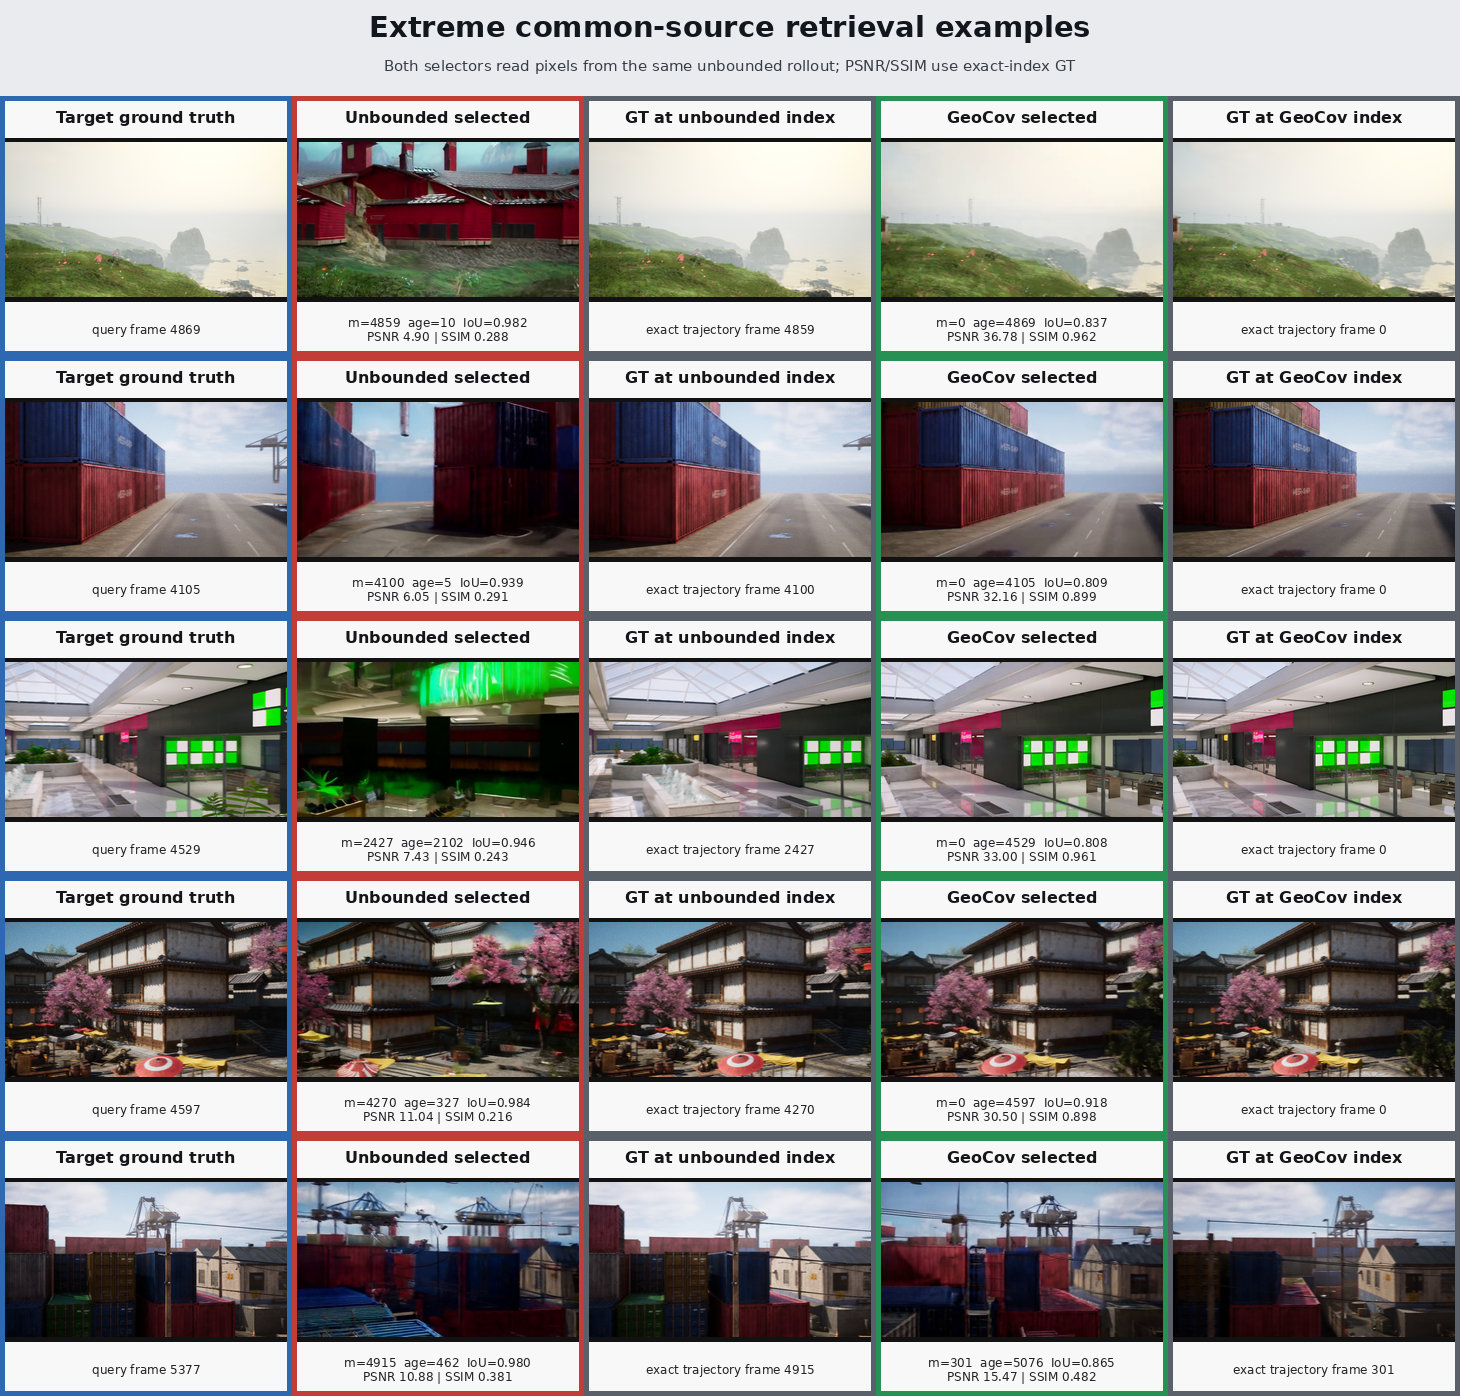
\includegraphics[width=0.82\textwidth]{figures/extreme_common_source_examples.png}
    \caption{\textbf{Large common-source retrieval disagreements.} Candidate
    pixels come from one complete-retention rollout; policies supply only the
    selected indices. Cases were chosen using high-overlap and fidelity-gap
    filters and illustrate possibilities rather than frequency.}
    \label{fig:extremes}
\end{figure}

\begin{figure}[!htbp]
    \centering
    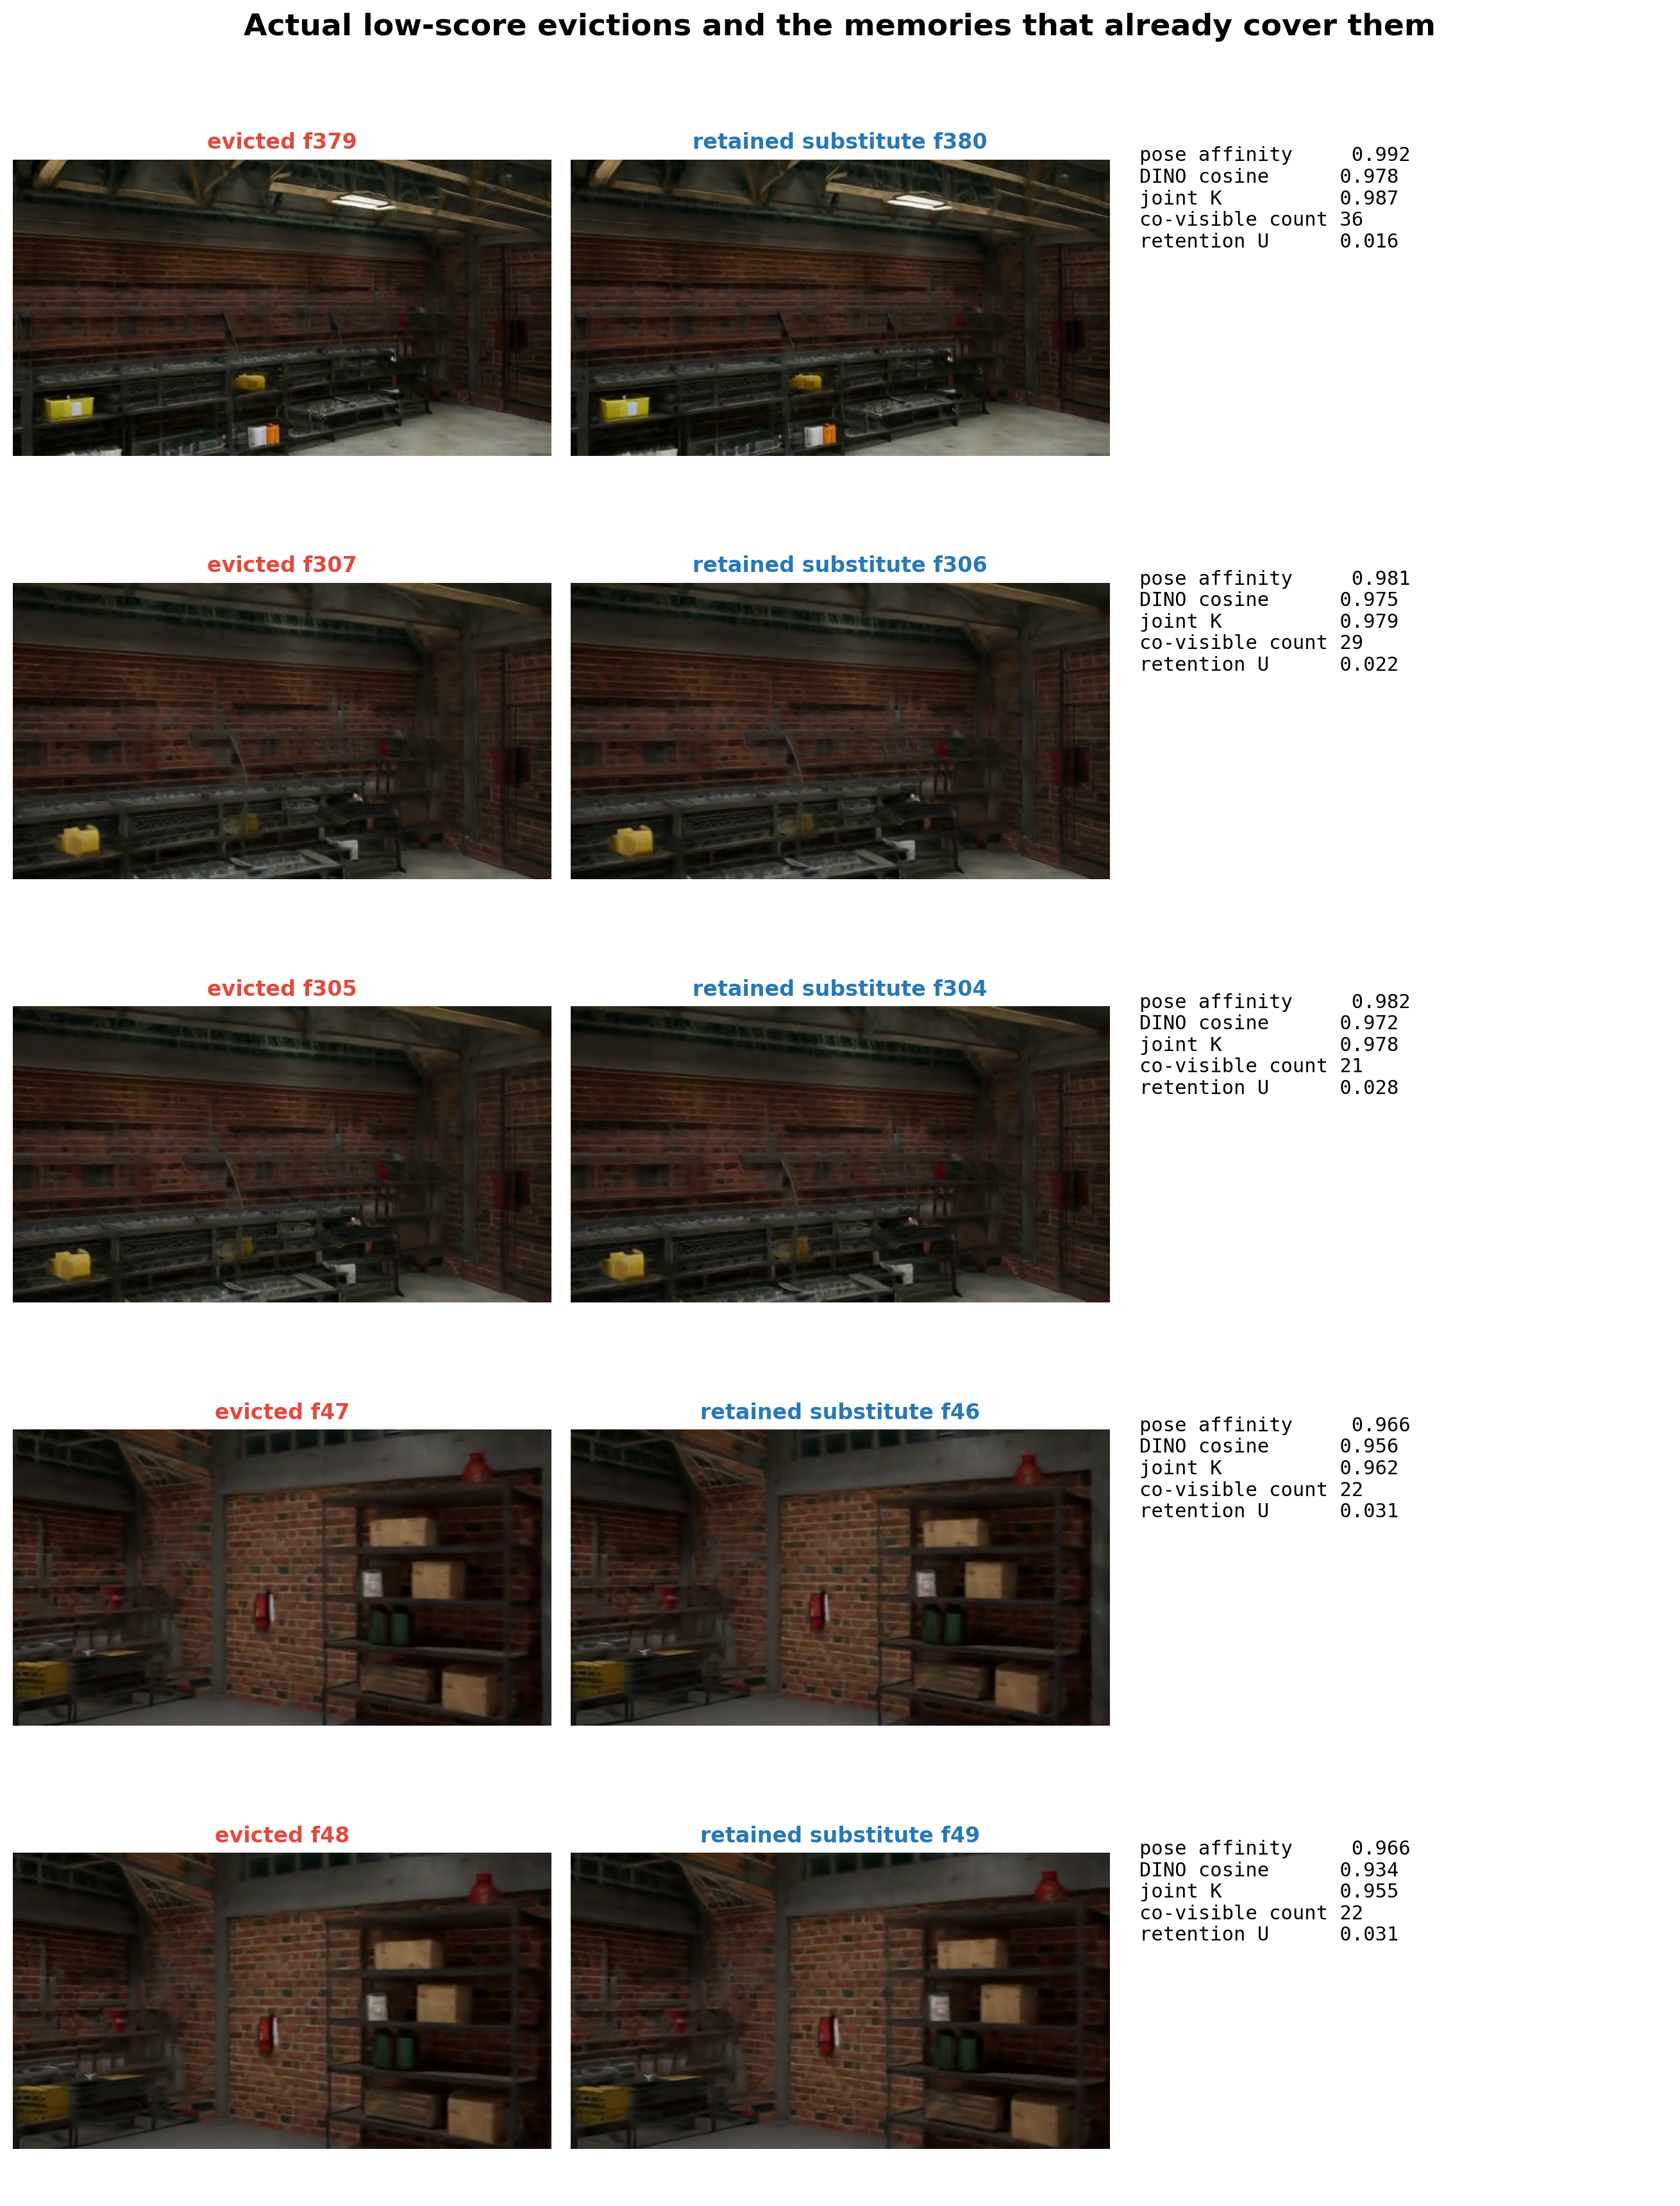
\includegraphics[height=0.78\textheight]{figures/geocov_evicted_substitutes.png}
    \caption{\textbf{Recorded evictions and retained substitutes.} In this
    Warehouse update, \Geo reduces 108 candidates to 32. Each displayed
    eviction has high pose affinity and DINO similarity to a retained neighbor;
    recomputed and logged eviction sets overlap by 97.4\%.}
    \label{fig:evictions}
\end{figure}

\FloatBarrier
\twocolumn
\bibliographystyle{plainnat}
\bibliography{references}

\end{document}
